\clearpage
\subsection{问题二的供需预测与方案选择}

问题二每天零点需要确定当天的普通购电量，而当天真实负载与光伏尚未出现。负载的星期规律较强，光伏则更适合参考近期变化，二者因而分别预测，再共同用于购电安排。预测只给出供需判断，储能能否弥补判断误差，以及弥补不了时需要支付多少紧急购电费，决定了策略的实际效果。

\subsubsection{分别建立负载与光伏预测}

设$\widehat L_{d,k}$和$\widehat P^{\mathrm{PV}}_{d,k}$分别为第$d$天零点对该日第$k$段的负载与光伏预测。首先建立同星期负载与近期光伏的历史平均模型：
\begin{equation}
 \widehat L_{d,k}=\frac{1}{a}\sum_{j=1}^{a}L_{d-7j,k},\qquad
 \widehat P^{\mathrm{PV}}_{d,k}=\frac{1}{b}\sum_{j=1}^{b}P^{\mathrm{PV}}_{d-j,k}.
 \label{eq:q2_history}
\end{equation}
其中$a$为采用的同星期历史日数，$b$为连续历史日数。负载只平均同类星期，避免把高、低负载日混在一起；光伏使用近期同刻平均，以跟随发电水平变化。历史不足时只平均当时已有样本，同星期样本为空时回退至最近可得历史。1月最初阶段若某一时刻尚无实际历史，则使用明确标记的附件1参考，不将其作为实测训练样本。

为检验是否需要更复杂的预测关系，另比较岭回归与梯度提升树。两者均分别拟合负载和光伏，输入包括日内位置、星期、目标日期、预测提前天数，以及各自此前的同刻、同星期和近期水平，不使用当天未来真实值。岭回归在标准化后的特征上估计系数：
\begin{equation}
 (\widehat\beta_0,\widehat{\boldsymbol\beta})=
 \arg\min_{\beta_0,\boldsymbol\beta}
 \left\{\sum_{i\in\mathcal T_d}
 (Y_i-\beta_0-\boldsymbol X_i^{\mathsf T}\boldsymbol\beta)^2
 +\lambda\lVert\boldsymbol\beta\rVert_2^2\right\}.
 \label{eq:q2_ridge}
\end{equation}
这里$Y_i$每次只取负载或光伏中的一个目标，$\mathcal T_d$仅包含第$d$天零点前已完整观测的训练目标。标准化参数与回归系数也只由该历史集合计算，截距不受惩罚。正则项限制短历史下过大的系数；系数可以为负，其含义是条件修正，不能当成加起来等于100\%的指标占比。

梯度提升树通过一系列小树逐步修正预测误差，其预测形式为
\begin{equation}
 \widehat f(\boldsymbol X)=f_0(\boldsymbol X)
 +\nu\sum_{m=1}^{M}h_m(\boldsymbol X),\qquad \nu=0.05,\quad M=200.
 \label{eq:q2_boosting}
\end{equation}
其中$h_m$为第$m$轮学得的修正，$\nu$控制每轮修正幅度。树的分裂位置和叶节点值由历史误差拟合，$\nu$是统一设置的学习步长，并非某个输入因素占5\%的权重。回归与树模型每七天更新一次，使用最近56个预测起点日中已能评分的样本。预测结果限制为非负，光伏还依据此前28天的同刻发电记录限制夜间输出；这一历史范围可能滞后于日出、日落时段的季节变化。

\subsubsection{权重、窗口与误差余量的确定}

式\eqref{eq:q2_history}在选定参考日后采用等权平均。各历史日与目标日的相似性先通过星期和近期窗口体现，再以等权保留共同轮廓，不仅凭某一天波动较大就赋予更高权重。历史数据的离散程度并不直接代表其预测价值，因此本文没有用熵权法决定这些日期的权重。

分别比较$a\in\{1,4\}$与$b\in\{3,7\}$的四种组合，以1月8日至31日按时间顺序回放得到的普通与紧急购电总费用选择窗口。所得$a=4$、$b=7$，即历史充足时，负载的四个同星期样本各占25\%，光伏的七个近期同刻样本各占$1/7$。这一选择有别于把负载和光伏按比例混成一条预测，两种功率仍分别估计。

在相同的历史回放条件下，岭回归的$\lambda$在1、10、100中选为100，提升树的最大深度在3、5、7中选为5。所有训练样本等权参与各自的拟合，不另外分配综合评价权重。窗口、正则强度和树深在2月比较开始前确定，后续只按既定频率更新系数或树，不用后来费用反改此前设置。

普通电价与五倍紧急电价使低估供需缺口的代价较高。为此，在历史平均预测上增加由既往实际误差确定的准备量。定义第$i$日第$k$段的净供需电量误差为
\begin{equation}
 \varepsilon_{i,k}=\big[(L_{i,k}-P^{\mathrm{PV}}_{i,k})
 -(\widehat L_{i,k}-\widehat P^{\mathrm{PV}}_{i,k})\big]\Delta t.
 \label{eq:q2_error}
\end{equation}
正值表示实际比预测更缺电。每日零点从过去28天已实现的误差中，按0--4、4--8、\ldots、20--24时六组构成经验误差集合$\mathcal E_{d,g}$，对同组时段采用
\begin{equation}
 b_{d,k}=\max\{0,\widehat Q_{\alpha}(\mathcal E_{d,g(k)})\},\qquad
 \widetilde E^{\mathrm L}_{d,k}=\widehat L_{d,k}\Delta t+b_{d,k}.
 \label{eq:q2_allowance}
\end{equation}
其中$\widehat Q_\alpha$是经验分位数，先对完整的有正有负误差取分位，再将负分位截为零。$b_{d,k}$是供计划使用的电量余量，单位为kWh，不是虚构的实际负载。历史为7--13天时合并日内各时段估计，不足7天时不加余量；四小时分组在历史不少于14天时启用。三档$\alpha=0.7,0.8,0.9$中，1月费用最低的是0.7；70\%表示经验分布的取值位置，不是购电比例，也不代表整天供电可靠率。

规划沿用储能的能量守恒、容量和充放功率约束，在零点考虑未来48小时，仅锁定其中当天的144段普通订单。第二天供需同样只参考当前可得历史。为体现截止时刻的剩余电量仍有后续用途，规划目标中采用每度内部储电$0.9p_1$元的末端参考价值；它只减少有限规划视野的放空倾向，不构成售电收益。实际运行按当前供需与库存充放电，电池仍不能补齐的缺口才紧急购电，实际费用始终为
\begin{equation}
 C=\sum_{d,k}p_kq_{d,k}+\sum_{d,k}5p_ke_{d,k},
 \label{eq:q2_actual_bill}
\end{equation}
其中$q_{d,k}$是零点订好的普通电量，$e_{d,k}$是实际紧急补购量。未接收的普通电仍按订单计费。费用系数由题给价格确定，不通过熵权法或人为评分重新分配。

\subsubsection{相同运行条件下的候选比较}

四条策略分别采用同星期历史平均、岭回归、提升树，以及同星期历史平均加误差余量。1月1日以问题一购电结构和6000 kWh初始库存启动；按本次时间解释缺少的首个实际区间，用附件1相应时段作初始化参考，其后使用附件2实际值。1月公共运行采用同星期负载与近3天光伏方法，四条比较策略均从其得到的2月1日库存\QTwoInitialStorage{} kWh开始，之后分别连续承接自身库存。它们使用相同的48小时规划与实际执行规则，白天不修改普通订单。区间内反馈以该段实际功率近似描述，不把实际供需提前提供给零点预测。

表\ref{tab:q2_compare}给出2月1日至6月30日150天的费用比较。光伏与负载预测精度分别计算，普通与紧急电费分别核算，再比较总费用。
\begin{inlinetable}
\caption{四条购电策略在2月至6月的费用比较}
\label{tab:q2_compare}
\begin{tabular}{lrrr}
\toprule 策略 & 普通费用/万元 & 紧急费用/万元 & 总费用/万元\\\midrule
同星期历史平均 & \QTwoBaseOrdinary & \QTwoBaseEmergency & \QTwoBaseTotal\\
岭回归 & \QTwoRidgeOrdinary & \QTwoRidgeEmergency & \QTwoRidgeTotal\\
梯度提升树 & \QTwoTreeOrdinary & \QTwoTreeEmergency & \QTwoTreeTotal\\
历史平均加误差余量 & \QTwoRiskOrdinary & \QTwoRiskEmergency & \QTwoRiskTotal\\
\bottomrule
\end{tabular}
\end{inlinetable}

提升树的负载平均绝对误差为130.72 kW，低于历史平均的153.62 kW，但光伏误差由168.20 kW增加到189.95 kW，其总费用仅比不加余量的历史方案略低。即使净供需平均误差较小，也不保证误差恰好发生在电池有能力缓冲的时段。岭回归在本次特征与参数范围内费用最高，这不足以否定所有回归方法，却说明复杂预测需要用实际购电后果证明价值。

误差余量方案与历史平均方案采用完全相同的负载和光伏预测，仅改变计划的准备量。其普通电费增加\QTwoOrdinaryIncrease{}万元，紧急电费减少\QTwoEmergencyReduction{}万元，总费用减少\QTwoSaving{}万元，降幅为\QTwoSavingPct{}\%；紧急购电量由23.39万度降至9.52万度。期末库存反而多出\QTwoStorageDifference{} kWh，因而该节费并非来自多消耗期末电量。基于这一同条件对照，本文选择历史平均加误差余量作为问题二当前采用的方案。

为观察节费是否集中在少数月份，进一步将总费用差额按月分解，如图\ref{fig:q2_cost}所示。
\begin{inlinefigure}
 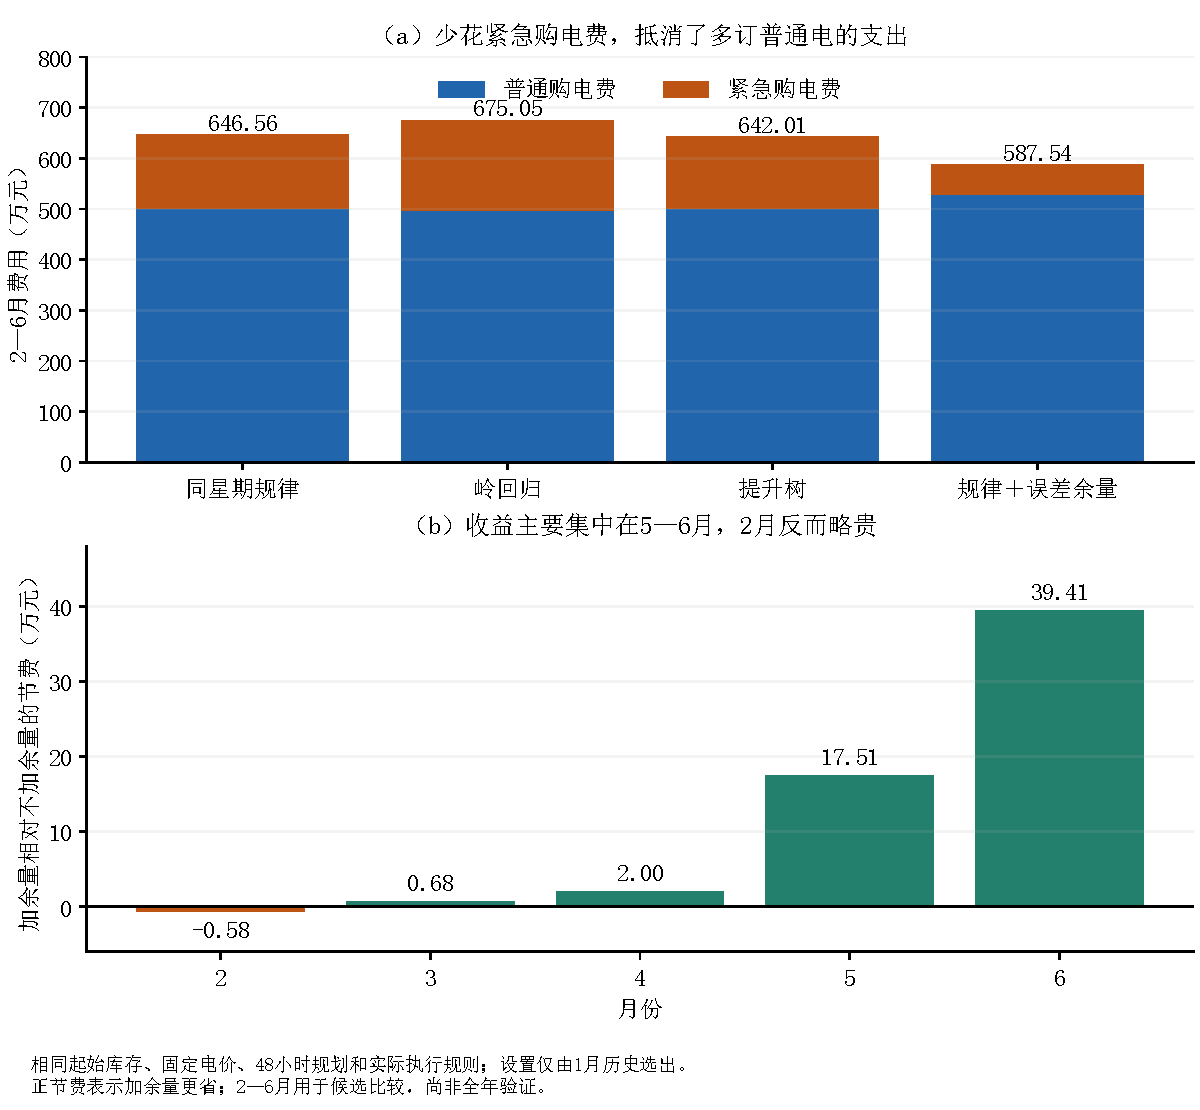
\includegraphics[width=0.88\linewidth]{q2_cost_and_months.pdf}
 \caption{候选策略的费用构成及误差余量方案的月度节费}
 \label{fig:q2_cost}
\end{inlinefigure}

余量方案并非每天都更省：150天中89天费用下降、45天增加、16天持平，2月累计多花0.58万元，而5月、6月分别少花17.51万元和39.41万元。1月参数回放中，三档正余量也均未超过零余量方案，0.7只是正余量候选中较便宜的一档。因此，余量的价值取决于供需偏差及电池所处状态，不能将本次结果概括为各月普遍占优。

多准备普通电也带来代价：相比不加余量，未接收但付费的普通电增加16.31万度，未利用光伏增加4.68万度。这些代价已反映在供电与费用账中。独立回读结果后，实际供需平衡和储电递推的最大残差均小于$10^{-9}$ kWh，全部订单与零点保存值一致；这些核查支持计算正确性，不替代其他季节、规划视野及余量参数的进一步验证。本次选择依据限定在上述150天、四条候选及共同执行规则，尚未构成全年最优性或普遍鲁棒性的证明。
